%%%%%%%%%%%%%%%%%%%%%%%%
%
% $Autor: Daanyaal Parvaize$
% $Datum: 2025-06-11 20:48:02Z $
% $Pfad: BA25-02-Time-Series/report/Contents/en/Test.tex
% $Version: 4621 $
%
% !TeX encoding = utf8
% !TeX root = Rename
%
%%%%%%%%%%%%%%%%%%%%%%%%

\chapter{Test For Software}

\section{Test Procedure}

Here we describe the standardized process to execute the tests, record results, and ensure test reproducibility.

\begin{enumerate}
	\item \textbf{Location of Tests:} All test scripts, including unit tests for individual functions, integration tests for model pipelines, and system tests for the complete application workflow, are located in the \texttt{test/} directory within the project root.
	
	\item \textbf{Executing Tests:} To execute the full test suite, navigate to the project root directory in a command-line interface and run the following command:
	
	\begin{framed}
		\begin{verbatim}
			pytest -v
		\end{verbatim}
	\end{framed}
	
	\item \textbf{Interpreting Results:} Upon completion, pytest outputs a summary report indicating the number of tests passed, failed, or skipped. Detailed error tracebacks are provided for failed tests to assist in debugging.
	
	\item \textbf{Re-running Specific Tests:} Individual tests or groups of tests can be run by specifying test file names or test function names to focus debugging efforts. For example:
	
	\begin{framed}
		\begin{verbatim}
			pytest test/test_data_loading.py
			pytest -k test_arima_training
		\end{verbatim}
	\end{framed}
	
	\item \textbf{Manual GUI Testing:} For interactive validation, the Streamlit app can be launched with:
	
	\begin{framed}
		\begin{verbatim}
			streamlit run app.py
		\end{verbatim}
	\end{framed}
	
	\item \textbf{Documentation of Test Runs:} All test runs, especially those related to release candidates, should be documented in a test log, including environment details, date/time, and any deviations observed.
\end{enumerate}


\section{Test Items}
\begin{itemize}
	\item \texttt{test\_arima.py}: ARIMA model training and failure scenarios
	\item \texttt{test\_config.py}: Configuration loading and saving tests
	\item \texttt{test\_data\_loader.py}: Data loading from CSVs, including date and wind speed parsing
	\item \texttt{test\_integration.py}: End-to-end ARIMA pipeline testing
	\item \texttt{test\_lstm.py}: LSTM model saving/loading and forecasting checks
	\item \texttt{test\_train\_script.py}: Model training from Jupyter-like scripts
\end{itemize}




\section{Test Cases and Results}

\footnotesize % Slightly smaller than \small
\begin{longtable}{|p{1.5cm}|p{3.8cm}|p{3.0cm}|p{3.3cm}|p{1.5cm}|}
	\hline
	\textbf{Test ID} & \textbf{Description} & \textbf{Input} & \textbf{Expected Output} & \textbf{Status} \\
	\hline
	\endfirsthead
	
	\hline
	\textbf{Test ID} & \textbf{Description} & \textbf{Input} & \textbf{Expected Output} & \textbf{Status} \\
	\hline
	\endhead
	
	TC01 & Load demo storm data & No file present & Generated demo CSV with valid wind speed and date columns & PASSED \\
	\hline
	TC02 & Load valid CSV & Sample \texttt{storms.csv} file & DataFrame with correct schema and data types & PASSED \\
	\hline
	TC03 & Wind speed numeric check & Sample storm data & \texttt{wind\_speed} column must be numeric & PASSED \\
	\hline
	TC04 & Date conversion check & Date string formats & All dates must convert to \texttt{datetime64} & PASSED \\
	\hline
	TC05 & ARIMA model training & Clean time series data & Model object fitted & PASSED \\
	\hline
	TC06 & ARIMA short data failure & \textless{} 10 data points & Should raise \texttt{ValueError} & PASSED \\
	\hline
	TC07 & LSTM model save/load & Trained model and scaler & Saved and reloaded models match & PASSED \\
	\hline
	TC08 & End-to-end ARIMA & Real data and model pipeline & Forecasts generated without error & PASSED \\
	\hline
	TC09 & Model training via script & Notebook-style script & Training completes & PASSED \\
	\hline
	TC10 & Data cleaning & CSV with missing \texttt{wind\_speed} & NaNs interpolated, column cleaned & PASSED \\
	\hline
\end{longtable}

\begin{figure}[H]
	\centering
	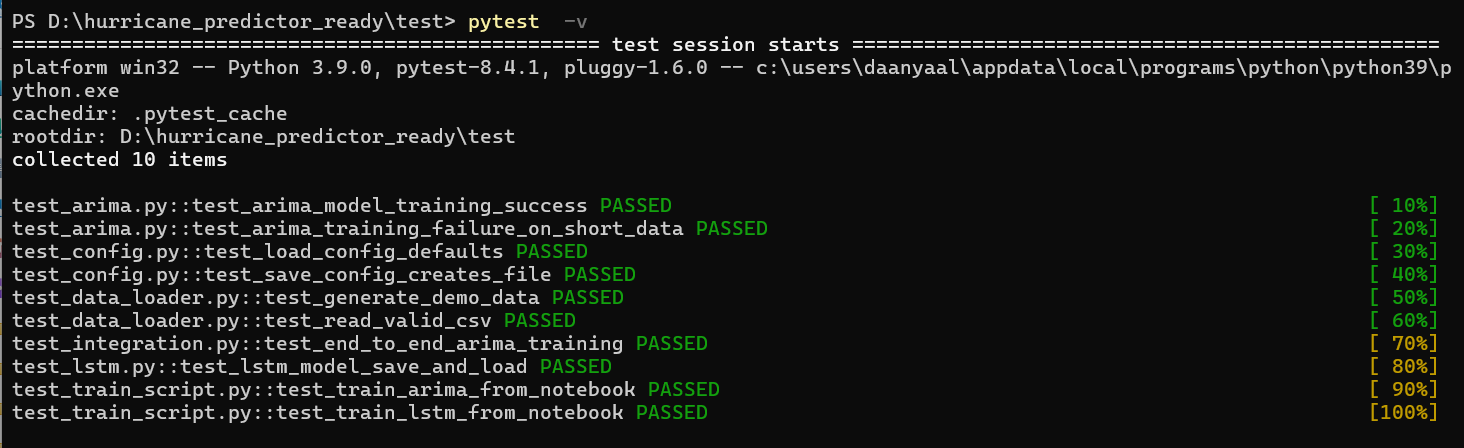
\includegraphics[width=1.2\textwidth, height=0.9\textheight, keepaspectratio]{../../BA25-02-Time-Series/report/Images/testoutput.png}
	\caption[Visualization of Test Output Results]{
		Visualization of the test output generated during the system validation phase.
	}
	\label{fig:testoutput}
\end{figure}










\section{Test Data}
The test data used in validating the Hurricane Intensity Predictor system is carefully selected and generated to cover a broad spectrum of real-world scenarios. This ensures the robustness and reliability of the system components.

\begin{itemize}
	\item \textbf{Auto-generated Demo Data:}  
	When no input file is found, the system automatically generates a demo dataset simulating typical hurricane wind speed measurements over a date range. This helps verify the data loading and preprocessing pipeline even without user-provided data.
	
	\item \textbf{Uploaded CSVs with Various Date Formats:}  
	The system is designed to handle diverse date formats commonly found in real-world storm datasets, including but not limited to:
	\begin{itemize}
		\item Partial dates without year, e.g., \texttt{09-Jun}, where the current year is assumed.
		\item Standard ISO formats, e.g., \texttt{2024/03/15} or \texttt{2023-01-01}.
		\item Separate year, month, and day columns that are combined into a unified datetime column.
	\end{itemize}
	This flexibility is critical since datasets from different sources vary widely in date representation.
	
	\item \textbf{Wind Speed Column Variability:}  
	The test inputs include CSV files with various wind speed column names, such as \texttt{wind}, \texttt{Wind Speed}, \texttt{Wind\_Spd}, etc. The system detects and standardizes these column names to \texttt{wind\_speed} internally, ensuring consistent downstream processing.
\end{itemize}

\section{Expected Results}
The test protocol defines clear expectations to validate correctness and user experience:

\begin{itemize}
	\item \textbf{System Stability:}  
	The application must not crash or throw unhandled exceptions upon uploading valid CSV files, regardless of date or column naming variations.
	
	\item \textbf{Accurate Forecast Generation:}  
	Both ARIMA and LSTM forecasting models must produce valid numeric wind speed predictions for the requested forecast horizon. The forecasts should be correctly aligned with the date indices.
	
	\item \textbf{Date Normalization:}  
	All date columns, including partial or non-standard formats, must be successfully converted into Python \texttt{datetime64} objects. When year information is missing, the system assigns the current year automatically without user intervention.
	
	\item \textbf{Visualization Consistency:}  
	The historical and forecasted wind speeds displayed on the Streamlit app’s plots must have correct axis labels and legends reflecting that the wind speed is measured in \textbf{knots}, the standard unit used in meteorological analyses.
\end{itemize}

\section{Reporting and Logging}
To facilitate effective debugging and quality control, the test execution environment incorporates the following practices:

\begin{itemize}
	\item \textbf{Console Output:}  
	Test results, including pass/fail status and error messages, are printed to the console or CI logs for immediate feedback.
	
	\item \textbf{Pytest Usage:}  
	The testing suite is executed using \texttt{pytest} with options \texttt{--maxfail=1} to stop after the first failure, \texttt{--disable-warnings} to suppress irrelevant warnings, and \texttt{-v} for verbose output. This balances thoroughness with manageable output.
	
	\item \textbf{Handling Deprecation Warnings:}  
	Current warnings related to deprecated Pandas methods such as \texttt{fillna(method=...)} are acknowledged and tracked for fixing in future updates to maintain codebase health and compatibility.
\end{itemize}

\section{Roles and Responsibilities}
Clear delineation of responsibilities ensures efficient testing and continuous integration:

\begin{itemize}
	\item \textbf{Developer:}  
	Responsible for writing, updating, and maintaining automated test scripts that cover unit, integration, and system-level tests. Developers run these tests locally before pushing code changes to prevent regressions.
	
	\item \textbf{Tester:}  
	Validates the correctness of test outputs, reviews test coverage for completeness, and performs exploratory manual testing using the Streamlit UI to catch edge cases not covered by automated tests.
\end{itemize}

\section{Schedule and Frequency}
To maintain project quality and reliability, the testing process follows a strict schedule:

\begin{itemize}
	\item \textbf{Milestone Testing:}  
	The full test suite is executed prior to every major project milestone or software release to ensure all system components work as expected.
	
	\item \textbf{Continuous Integration:}  
	Critical tests—specifically those covering data loading, ARIMA model training, and LSTM forecasting—must pass on every push or pull request to the repository. This enforces stability in the core forecasting pipeline.
	
	\item \textbf{Periodic Regression Testing:}  
	Additional non-critical tests and UI checks are run weekly or as needed to detect subtle issues arising from incremental changes.
\end{itemize}

\section{Automation Guide}

This section provides a detailed, step-by-step guide for users and developers on how to run the automated test suite designed for the Hurricane Intensity Predictor project. Automation plays a vital role in ensuring the software remains reliable, stable, and bug-free throughout development, testing, and deployment.

\subsection{Purpose of Automation}

Automated testing helps us verify that every part of the system—from small individual functions to the full integrated application—works as intended. By automating tests, we avoid repetitive manual checks, save valuable time, and quickly detect if new changes introduce bugs or errors. This continuous verification process is essential for maintaining high-quality software that users can trust.

\subsection{Prerequisites}

Before you start running tests, make sure your environment meets the following conditions:

\begin{itemize}
	\item \textbf{Python Installation:} Python version 3.9 is recommended, as the project dependencies are tested with this version.
	\item \textbf{Project Dependencies:} All required Python libraries should be installed. This is handled via a \texttt{requirements.txt} file included in the project.
	\item \textbf{Command-Line Access:} You should be comfortable opening and using a terminal, PowerShell, or command prompt window on your computer.
\end{itemize}

\subsection{Setup Instructions}

Follow these steps to prepare your local environment for running automated tests:

\begin{enumerate}
	\item \textbf{Clone the Project Repository:}
	\begin{framed}
		\begin{verbatim}
			git clone <repository_url>
			cd <repository_folder>
		\end{verbatim}
	\end{framed}
	Replace \texttt{<repository\_url>} with the actual URL of the GitHub repository, and \texttt{<repository\_folder>} with the folder name that gets created.
	
	\item \textbf{Create and Activate a Virtual Environment (Optional but Recommended):}
	\begin{framed}
		\begin{verbatim}
			python -m venv venv
			source venv/bin/activate    # On Linux or macOS
			venv\Scripts\activate       # On Windows
		\end{verbatim}
	\end{framed}
	Using a virtual environment keeps the project’s dependencies isolated from other Python projects on your system, avoiding version conflicts.
	
	\item \textbf{Install Project Dependencies:}

	\begin{lstlisting}[language=bash, basicstyle=\ttfamily\small]
		pip install --upgrade pip
		pip install -r application/hurricane_predictor_ready/requirements.txt
	\end{lstlisting}





	This command reads the \texttt{requirements.txt} file and installs all necessary Python packages needed for the project and testing.
\end{enumerate}

\subsection{Running the Automated Tests}

Once your environment is ready, run the tests using the following steps:

\begin{enumerate}
	\item \textbf{Go to the Project Root Folder:}
	\begin{framed}
		\begin{verbatim}
			cd <repository_folder>
		\end{verbatim}
	\end{framed}
	
	\item \textbf{Run the Full Test Suite:}
	\begin{framed}
		\begin{verbatim}
			pytest -v
		\end{verbatim}
	\end{framed}
	This command executes all tests found in the project’s \texttt{test/} directories. The \texttt{-v} flag means “verbose,” so you will see detailed output for each test, including its name and whether it passed or failed.
	
	\item \textbf{Run Specific Tests for Faster Debugging:}
	If you want to test only a specific file or function (to save time during debugging), use these commands:
	\begin{framed}
		\begin{verbatim}
			pytest test/test_data_loading.py
			pytest -k test_arima_training
		\end{verbatim}
	\end{framed}
	
	\item \textbf{Understand Test Results:}
	After running, look at the console output:
	\begin{itemize}
		\item \texttt{PASSED} means the test succeeded.
		\item \texttt{FAILED} means the test found a problem; traceback information helps locate the error.
		\item \texttt{SKIPPED} means the test was intentionally not run, often due to conditions not met.
	\end{itemize}
	
	\item \textbf{Stop Testing on First Failure (Optional):}
	To save time during development, you can stop the test run as soon as the first failure occurs by running:
	\begin{framed}
		\begin{verbatim}
			pytest --maxfail=1 -v
		\end{verbatim}
	\end{framed}
\end{enumerate}

\subsection{Manual GUI Testing}

Besides automated tests, it is important to manually check the interactive application interface to ensure everything behaves as expected from a user’s perspective:

\begin{framed}
	\begin{verbatim}
		streamlit run application/hurricane_predictor_ready/app.py
	\end{verbatim}
\end{framed}

This command launches the Streamlit web application locally, where you can upload hurricane data files, generate forecasts, and visually inspect the plots and results.

\subsection{Recommended Continuous Integration}

For professional development workflows, automated testing is usually integrated with version control platforms like GitHub. This project is configured (or can be configured) to run all tests automatically on every code push or pull request using GitHub Actions. This continuous integration (CI) setup helps catch bugs early and maintain code quality without manual intervention. If not already active, it is recommended to set up CI in a future update.



\subsection{Automation Flowchart}
		\begin{figure}[h!]
		\centering
		\begin{tikzpicture}[node distance=1.5cm and 0cm,
			startstop/.style={
				rectangle, rounded corners, minimum width=5cm, minimum height=1cm,
				text centered, draw=black, fill=red!30, font=\sffamily\small
			},
			process/.style={
				rectangle, minimum width=5cm, minimum height=1cm,
				text centered, draw=black, fill=blue!20, font=\sffamily\small
			},
			arrow/.style={
				thick, ->, >=Stealth
			}
			]
			
			% Nodes
			\node (clone) [startstop] {Clone the Project Repository};
			\node (venv) [process, below=of clone] {Create \& Activate Virtual Environment (Optional)};
			\node (install) [process, below=of venv] {\parbox{5cm}{Install Dependencies \\ (using \texttt{requirements.txt})}};
			\node (runall) [process, below=of install] {\parbox{5cm}{Run Full Test Suite \\ \texttt{pytest -v}}};
			\node (runpart) [process, below=of runall] {\parbox{5cm}{Run Specific Tests (optional) \\ \texttt{pytest test\_file.py}}};
			\node (interpret) [process, below=of runpart] {Interpret Test Results};
			\node (manual) [process, below=of interpret] {\parbox{5cm}{Manual GUI Testing with Streamlit \\ \texttt{streamlit run app.py}}};
			\node (ci) [process, below=of manual] {\parbox{5cm}{Automatic Testing on GitHub \\ via Continuous Integration}};
			\node (end) [startstop, below=of ci] {\parbox{5cm}{Automation Ensures Reliable \\ \& Efficient Testing}};
			
			% Arrows
			\draw [arrow] (clone) -- (venv);
			\draw [arrow] (venv) -- (install);
			\draw [arrow] (install) -- (runall);
			\draw [arrow] (runall) -- (runpart);
			\draw [arrow] (runpart) -- (interpret);
			\draw [arrow] (interpret) -- (manual);
			\draw [arrow] (manual) -- (ci);
			\draw [arrow] (ci) -- (end);
			
		\end{tikzpicture}
		\caption{Automation Guide Flowchart}
		\label{fig:automation_flow}
	\end{figure}
	
	
	





